

\section{Coeficiente de empuje} % (fold)
\label{sec:parte1}

\question{Explicar en pocas palabras 3 posibles métodos pasa calcular el empuje adicional causado por sobrecargas externas}{
	\begin{itemize}[label=\ding{69}]
		\item Uniforme:
		\begin{figure}[H]
			\centering
			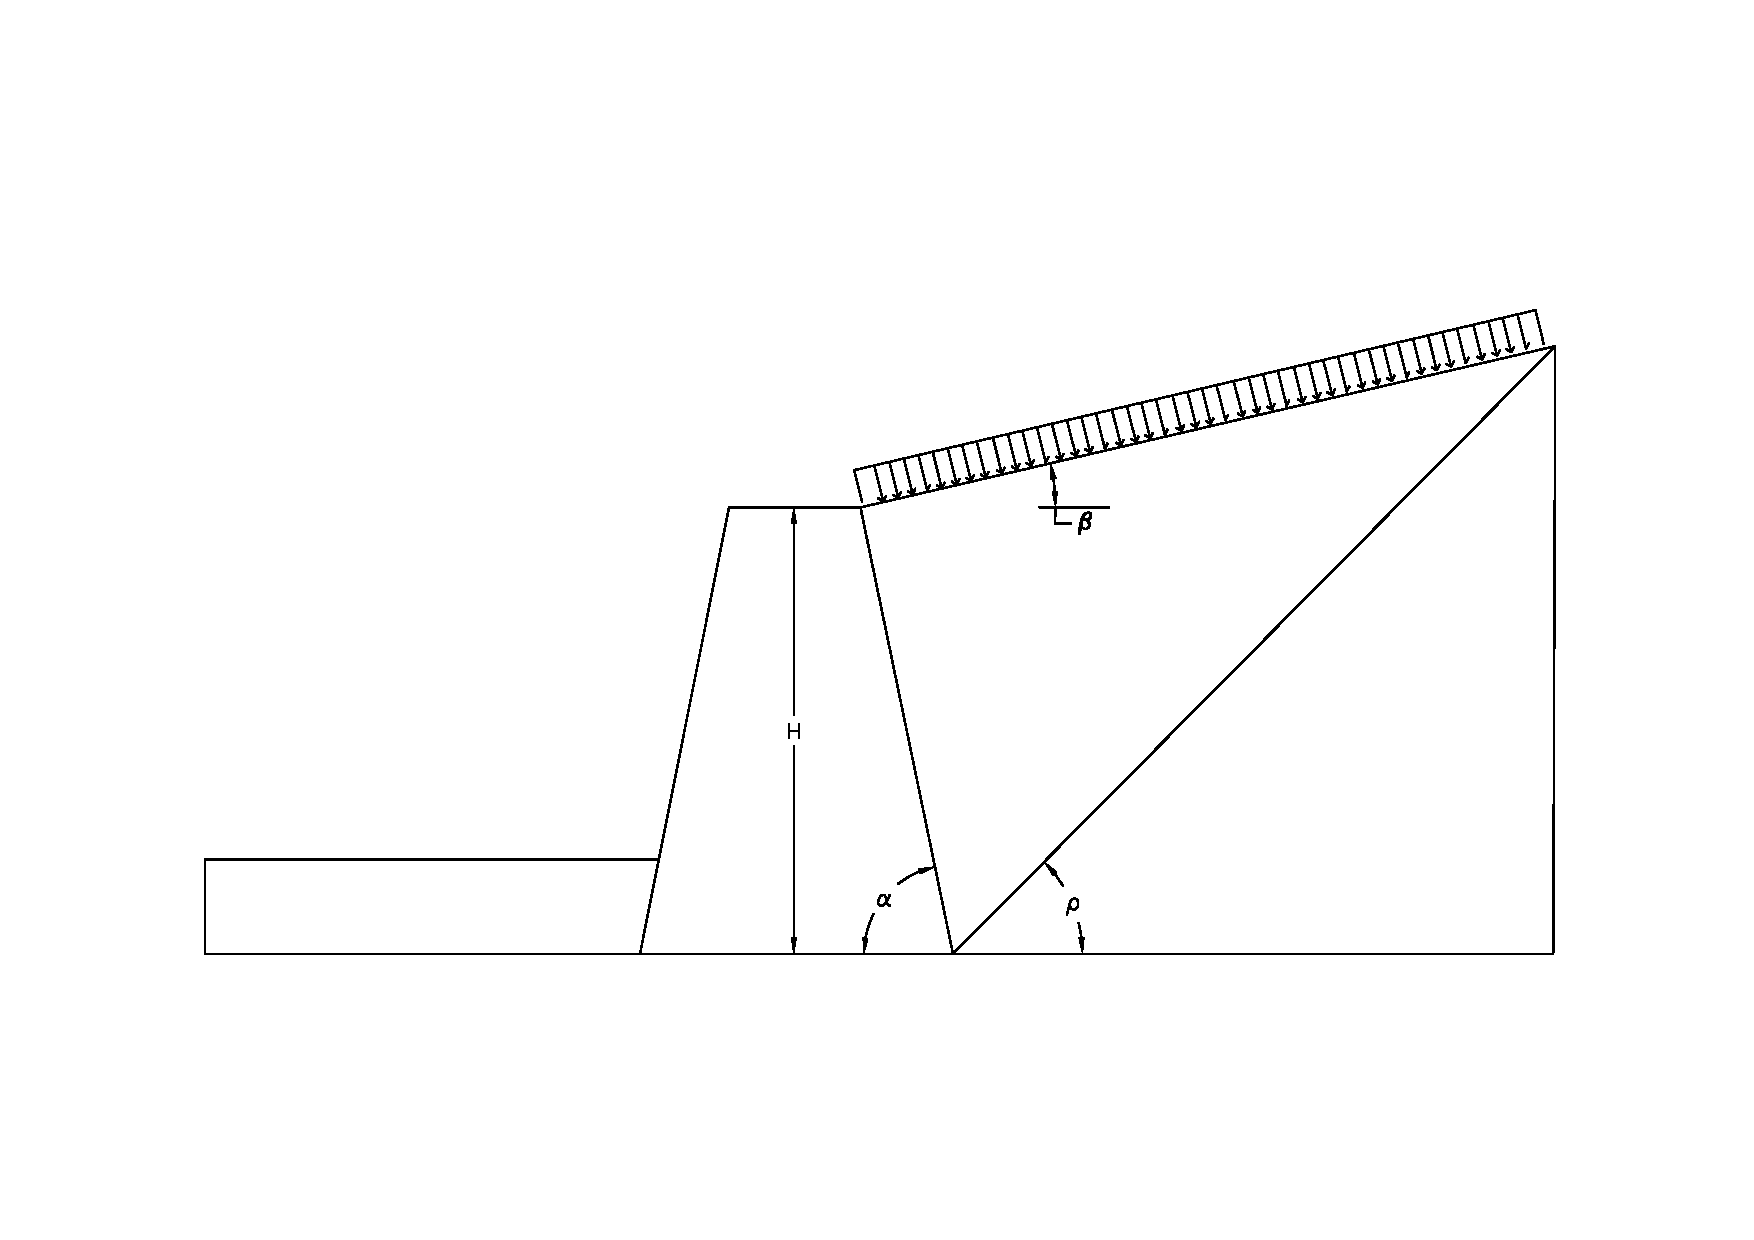
\includegraphics[width=0.7\textwidth]{img/cargas_uni}
			\caption{caption}
			\label{fig:Cargas uniformes}
		\end{figure}
		\[
			\gamma^{eq} = \gamma \frac{2q \sin(\alpha)}{H \sin(\alpha + \beta)}, \quad \emph{una densidad equivalente}
		\]
		O bien
		\[
			\Delta H = \frac{q \sin(\alpha)}{H \sin(\alpha+\beta)}, \quad \emph{una altura equivalente}
		\]
		\item No uniforme:
		\begin{figure}[H]
			\centering
			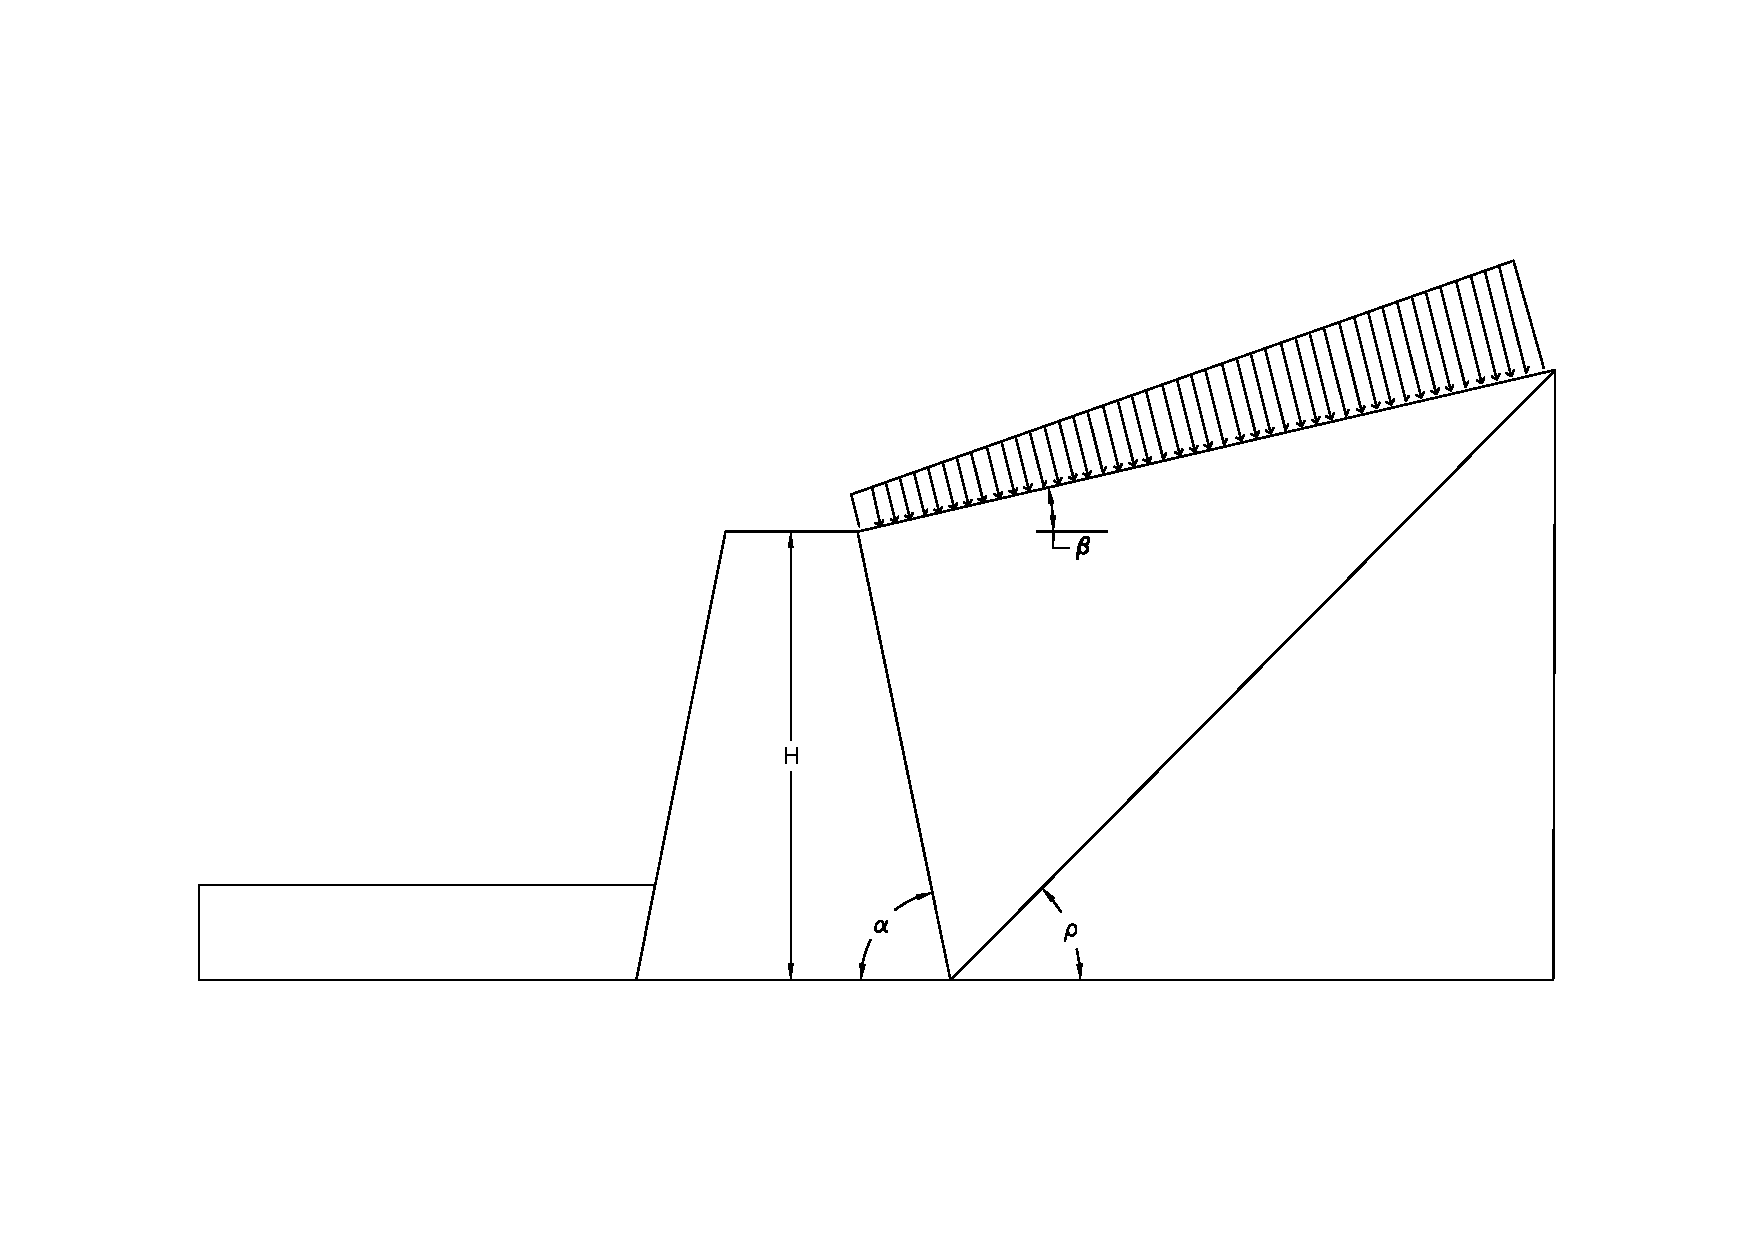
\includegraphics[width=0.7\textwidth]{img/cargas_no_uni}
			\caption{Cargas no uniformes}
			\label{fig:label}
		\end{figure}
		\begin{itemize}[label=\ding{71}]
			\item Soluciones elásticas (Boussinesq)
			\item Soluciones plásticas
			\item Reglas empíricas
		\end{itemize}
	\end{itemize}
}

\question{ Un muro con alto ángulo de rozamiento (40) está en contacto con un suelo de ángulo de fricción igual a 30. a) ¿ Qué valor escogerías como ángulo de rozamiento suelo-muro ? }{
	a)
	\[
		\delta = \frac{2}{3} \phi^{’}= 20
	\]
	b)
}

\question{¿ Qué diferencia conceptual existe entre el método de Coulomb y el de Rankine para el cálculo de empuje de tierras ? }{
	\begin{itemize}[label=\ding{69}]
		\item Rankine: 
		\begin{enumerate}
			\item no se considera rozamiento suelo-muro ($\delta=0$)
			\item se supone rotura completa del suelo
		\end{enumerate}
		\item Coulomb:
		\begin{enumerate}
			\item consideramos rozamiento suelo-muro ($\delta \neq 0$)
			\item Rotura según 2 planos, uno de ángulo $\rho$ y otro con el muro
		\end{enumerate}
	\end{itemize}
}

\question{Enumerar las razones por las que el metodo de Rankine es más seguro que el de Coulomb para el cálculo de empujes de tierras.}{
	\begin{enumerate}
		\item En el caso \textbf{pasivo} no es aconsejable usar Coulomb, pues sobre-estima lo que va a resistir el terreno 
		\[
			K_{pc}>K_{p-real} \Rightarrow E_{pc}>E{p-real}
		\]
		\item Rankine supone $\delta = 0 \Rightarrow$ \textbf{empuje activo máximo} ($\nexists$ componente estabilizadora del empuje) en la teoría de Coulomb supone parte del empuje como estabilizador 
		\[
		 	E_{Rankine} > E_{Coulomb}
		 \] 
		 \item Rankine supone rotura en todo el terreno, mientra Coulomb solo la considera en 2 lineas.
	\end{enumerate}
	Así pues el terreno rompe antes de lo que dica Coulomb.
}

\question{Cúal es la influencia de la fricción suelo-muro sobre: 
\begin{itemize}[label=\ding{69}]
	\item Empuje activo
	\item Empuje pasivo
	\item $K_0$
	\item Momento de vuelco por empuje activo
\end{itemize}}{
	\begin{itemize}[label=\ding{69}]
		\item \emph{Empuje activo:}
		\[
			\delta \approx \frac{2}{3} \phi^{’}
		\] 
		y 
		\[
			K_a = \frac{1- \sin(\phi^{’})}{1+ \sin(\phi^{’})} \Rightarrow \frac{\dif K_a}{\dif\phi^{’}}<0
		\]
		Con lo cual 
		\[
			\frac{\dif E_a}{\dif\delta}<0
		\]
		\item \emph{Empuje pasivo:}
		\[
			K_p = \frac{1+ \sin(\phi^{’})}{1+ \sin(\phi^{’})} \Rightarrow \frac{\dif K_a}{\dif\phi^{’}}>0
		\]
		Con lo cual 
		\[
			\frac{\dif E_p}{\dif\delta}>0
		\]
		\item $K_0$:
		No influye al estar en reposo
		\item \emph{Momento de vuelco por empuje activo}:
		\[
			\frac{\dif E_a}{\dif\delta}<0 \Rightarrow \frac{\dif M}{\dif\delta}<0
		\]
	\end{itemize}
}

\question{Dibujar cualitativamente la ley de empujes de Rankine sobre el muro de la Figure~\ref{fig:emp_gravedad}}{
	\begin{figure}[H]
		\centering
		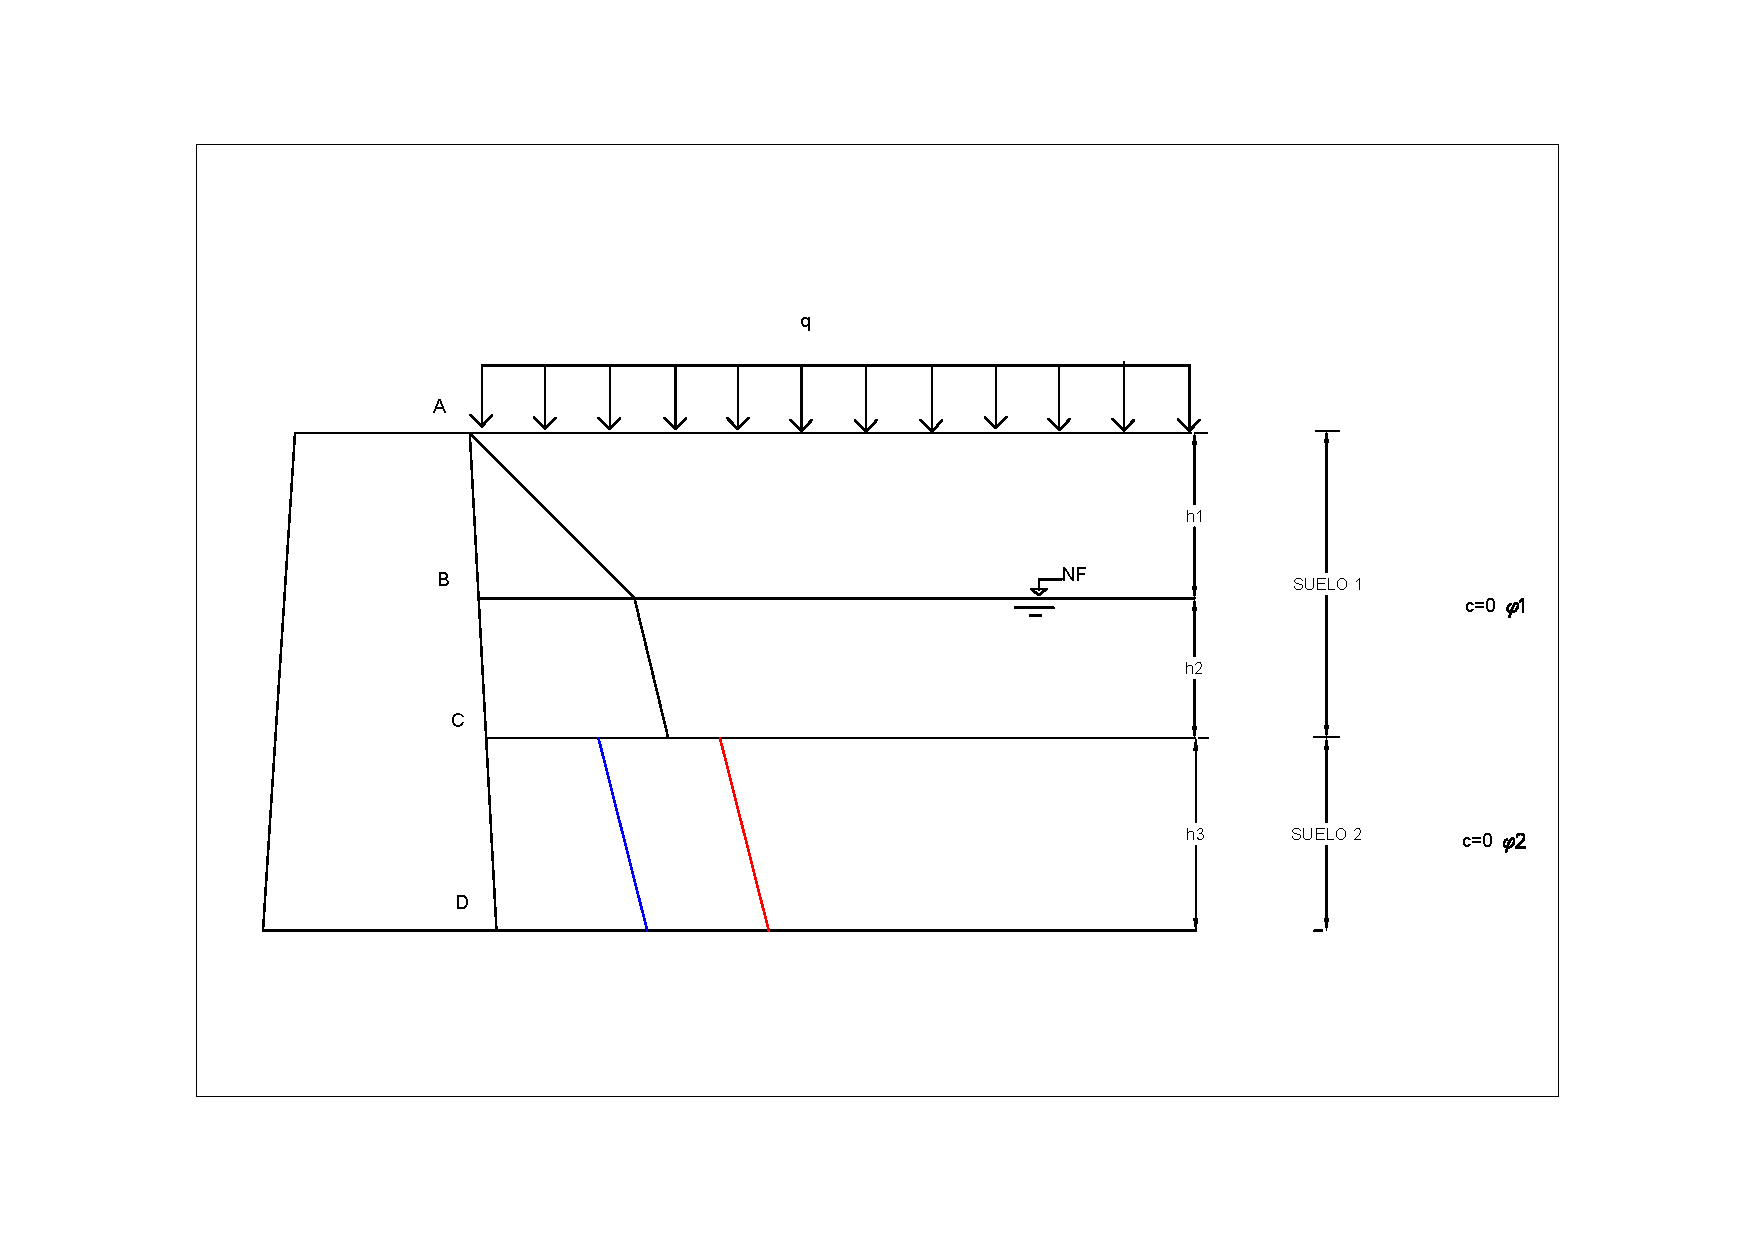
\includegraphics[width=0.9\textwidth]{img/ejemplo_empuje}
		\caption{Empuje de tierras sobre muro de gravedad}
		\label{fig:emp_gravedad}
	\end{figure}
	Tenemos:
	\begin{itemize}
		\item A: 
		\[
			\sigma_v^{’} = 0 \Rightarrow \sigma_h^{’}=0
		\]
		\item B:
		\[
			\sigma_v^{’} = \gamma h_1 + q \Rightarrow \sigma_h^{’}= K_a(\gamma h_1 + q)
		\]
		\item C:\\
		\emph{Parte superior:}
		\[
			\sigma_v^{’} = \gamma h_1 + \gamma^{’}h_2 + q \Rightarrow \sigma_h^{’}= K_a^{\phi_1}(\gamma h_1 + \gamma^{’}h_2+ + q)
		\]
		\emph{Parte inferior:}
		\[
			\sigma_v^{’} = \gamma h_1 + \gamma^{’}h_2 + q \Rightarrow \sigma_h^{’}= K_a^{\phi_2}(\gamma h_1 + \gamma^{’}h_2+ + q)
		\]
		\item D:
		\[
			\sigma_v^{’} = \gamma h_1 + \gamma^{’}(h_2+ h_3) + q \Rightarrow \sigma_h^{’}= K_a^{\phi_2}(\gamma h_1 + \gamma^{’}(h_2+ h_3) + q)
		\]

		\begin{myrem}
			En rojo el caso en el que $\phi_2 < \phi_1$ y en azul el contrario. En efecto tenemos $\frac{\dif K_a}{\dif\phi^{’}}>0$. Luego la variación de pendiente se debe a $\gamma^{’} < \gamma$
		\end{myrem}
	\end{itemize}
}

\question{Indicar qué parametros o propiedades fundamentales del terreno controlan el valor de $K_0$. ¿ Cómo varía $K_0$ con ellos ?}{

	EL grado de consolidación, $\phi^{’}$ y $I_p$. En el caso de tener una arcilla NC podemos considerar $K_0 = 1 - \sin(\phi^{’})$.

	\begin{minipage}{0.5\linewidth}
		\begin{figure}[H]
		\centering
		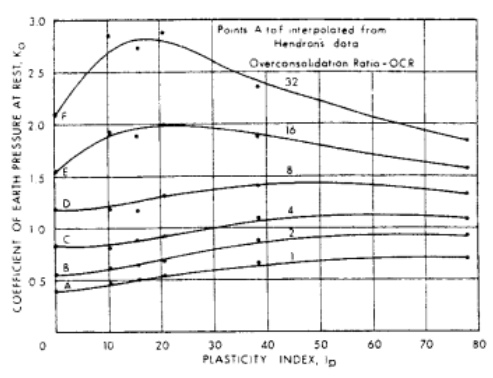
\includegraphics[width=\textwidth]{img/im1}
		\caption{caption}
		\label{fig:label}
		\end{figure}
	\end{minipage}%
	\begin{minipage}{0.5\linewidth}
		\begin{figure}[H]
			\centering
			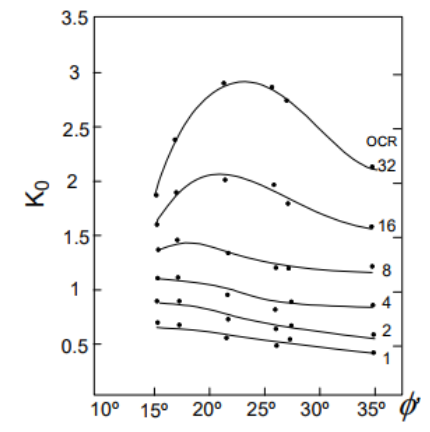
\includegraphics[width=\textwidth]{img/im3}
			\caption{caption}
			\label{fig:label}
		\end{figure}
	\end{minipage}
	
	\begin{figure}[H]
		\centering
		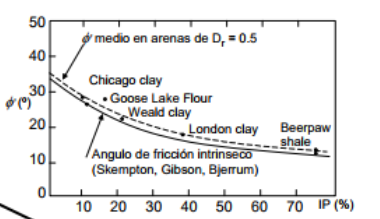
\includegraphics[width=0.5\textwidth]{img/im2}
		\caption{caption}
		\label{fig:label}
	\end{figure}
}

\question{¿ Cómo determinarías $K_0$ en laboratorio ? }{
	\begin{itemize}
		\item Ensayos edometricos
		\item Evaluación mediante succión (atención a la disminución de humedad)
	\end{itemize}
}

\question{ ¿ Podrías mencionar algún error conceptual que se admite en el desarollo del método del círculo de fricción para el cálculo del empuje pasivo ? Razonar para el caso c=0}{
	En el caso de empule pasivo en arcillas a largo plazo (c=0). Calcularemos el empuje pasivo como la suma de 2 estados:
	\begin{enumerate}
		\item Sólo interviene el peso sin cohesión $E_p^1$
		\item Sólo interviene la cohesión y el rozamiento del suelo, no interviene el peso $E_p^2$
	\end{enumerate}
	Luego $E_{total}=E_p^1+E_p^2$. Este procedimiento comporta errores:
	\begin{enumerate}
		\item Utilizo el método de estados límites de rotura $\rightarrow$ no se debe utilizar la superposición de estados.
		\item La superficie de rotura del estado 1 no tiene porque coincidir con la del estado 2.
	\end{enumerate}
	Estos errores se compensan ya que este metodo da resultados aceptables.
}

\question{ ¿ Están del lado de la seguridad los empujes pasivos alcanzados según Coulomb ?}{
	No, ya que sobre-estiman el empuje del suelo (al tener en cuenta el rozamiento).
}

\question{ ¿ Para movilizar $K_a$ son necesarias mayores $\varepsilon$ que para $K_p$ ?}{
	No, es al revés.
	\begin{figure}[H]
		\centering
		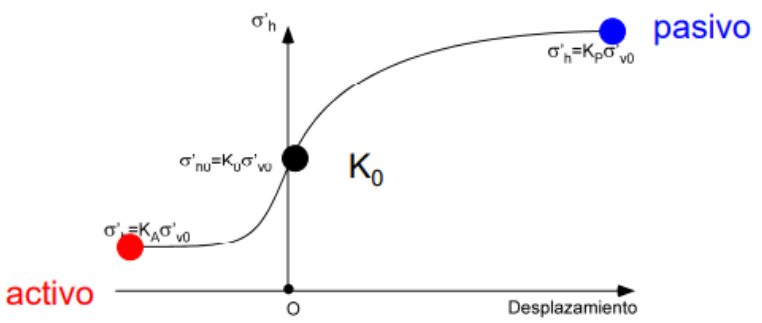
\includegraphics[width=0.5\textwidth]{img/im4}
		\caption{caption}
		\label{fig:label}
	\end{figure}

}

\question{¿ Puede darse el caso de que Coulomb prediga unas condiciones más desfavorables que Rankine en el caso activo ?}{
	No, ya que al considerar el rozamiento parte del empuje es estabilizador.
}

\question{ Hipótesis y utilización de la fórmula de Rankine }{
	\begin{enumerate}
		\item Todo el suelo esta en rotura
		\item La superficie de rotura es plana
		\item Rozamiento suelo/muro es nulo $\Rightarrow$ Tensiones principales
	\end{enumerate}
	Uso:
	\begin{enumerate}
		\item Trasdós vertical
		\item Terreno horizontal o inclinado un ángulo $\beta$
	\end{enumerate}
}

\question{Hipótesis de Coulomb para la determinación del empuje activo}{
	\begin{enumerate}
		\item Rotura plana: las lineas de contorno están en rotura 
		\item ``Suelo no cohesivo (c’=0) $\rightarrow$ friccional''
		\item ``No existen cargas aplicadas en superficie''
		\item Suelo homogéneo
		\item Suelo isotropo
		\item ``No hay agua $\rightarrow$ suelo seco''
	\end{enumerate}
}

\question{ En que casos se puede utilizar la teoría de Coulomb para la determinación del empuje pasivo ? Razonar}{
	Coulomb sobre-valora el empuje pasivo al considerar el rozamiento. Supone roturas planas cuando en realidad son curvas. Cúanto mayor sea $\delta$ mayor la distancia con la realidad.
}


% section questions (end)